\section{Sistema C – Sistema Acesso ao Estacionamento}

\begin{figure}[H]
    \centering
    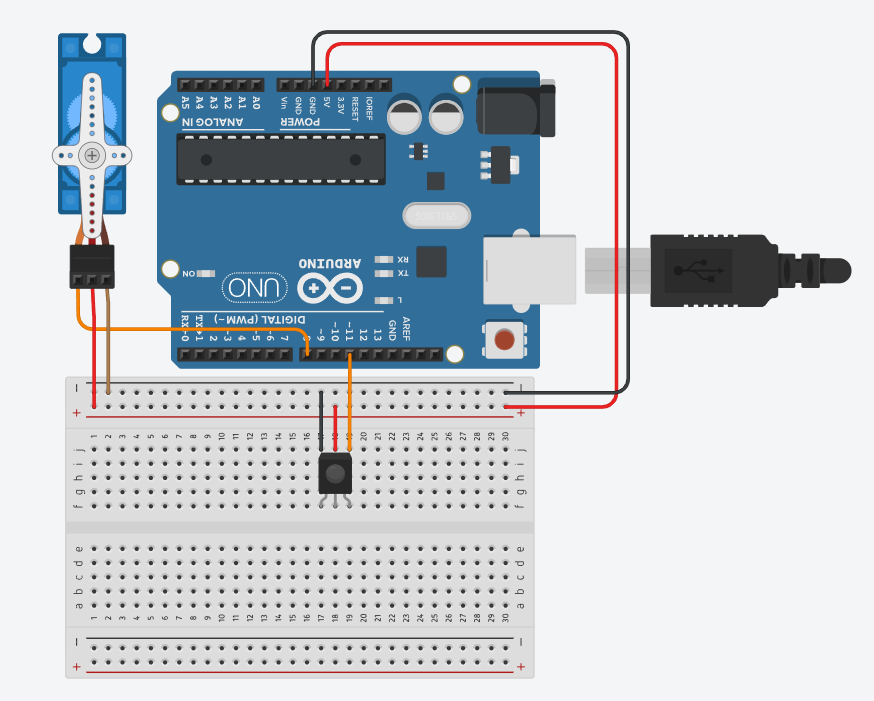
\includegraphics[scale=0.4]{images/hardware/sisC_tinkercad.png}    
    \selectlanguage{portuguese}\caption{Esquema do Sistema C}
\end{figure}

\begin{figure}[H]
\centering
\setlength{\arrayrulewidth}{0.5mm}
\renewcommand{\arraystretch}{1.5}
\begin{tabular}{|l | c|} 
 \hline
 \multicolumn{1}{|c|}{Componentes} & \multicolumn{1}{|c|}{Quantidade}\\ [0.8ex] 
 \hline
 Sensor Infravermelhos & 1x \\ 
 \hline
 Motor Servo & 1x \\
 \hline
 Arduino & 1x \\
 \hline
 Breadboard & 1x\\
 \hline
 Comando Infravermelhos & 1x  \\ 
 \hline
\end{tabular}
\selectlanguage{portuguese}\caption{Componentes Utilizados}
\end{figure}


O Sensor infravermelhos encontra-se ligado à porta nº 11 para envio dos dados.

O motor Servo encotra-se ligado à porta nº 8 para ser controlado pelo arduino.



\begin{figure}[H]
    \centering
    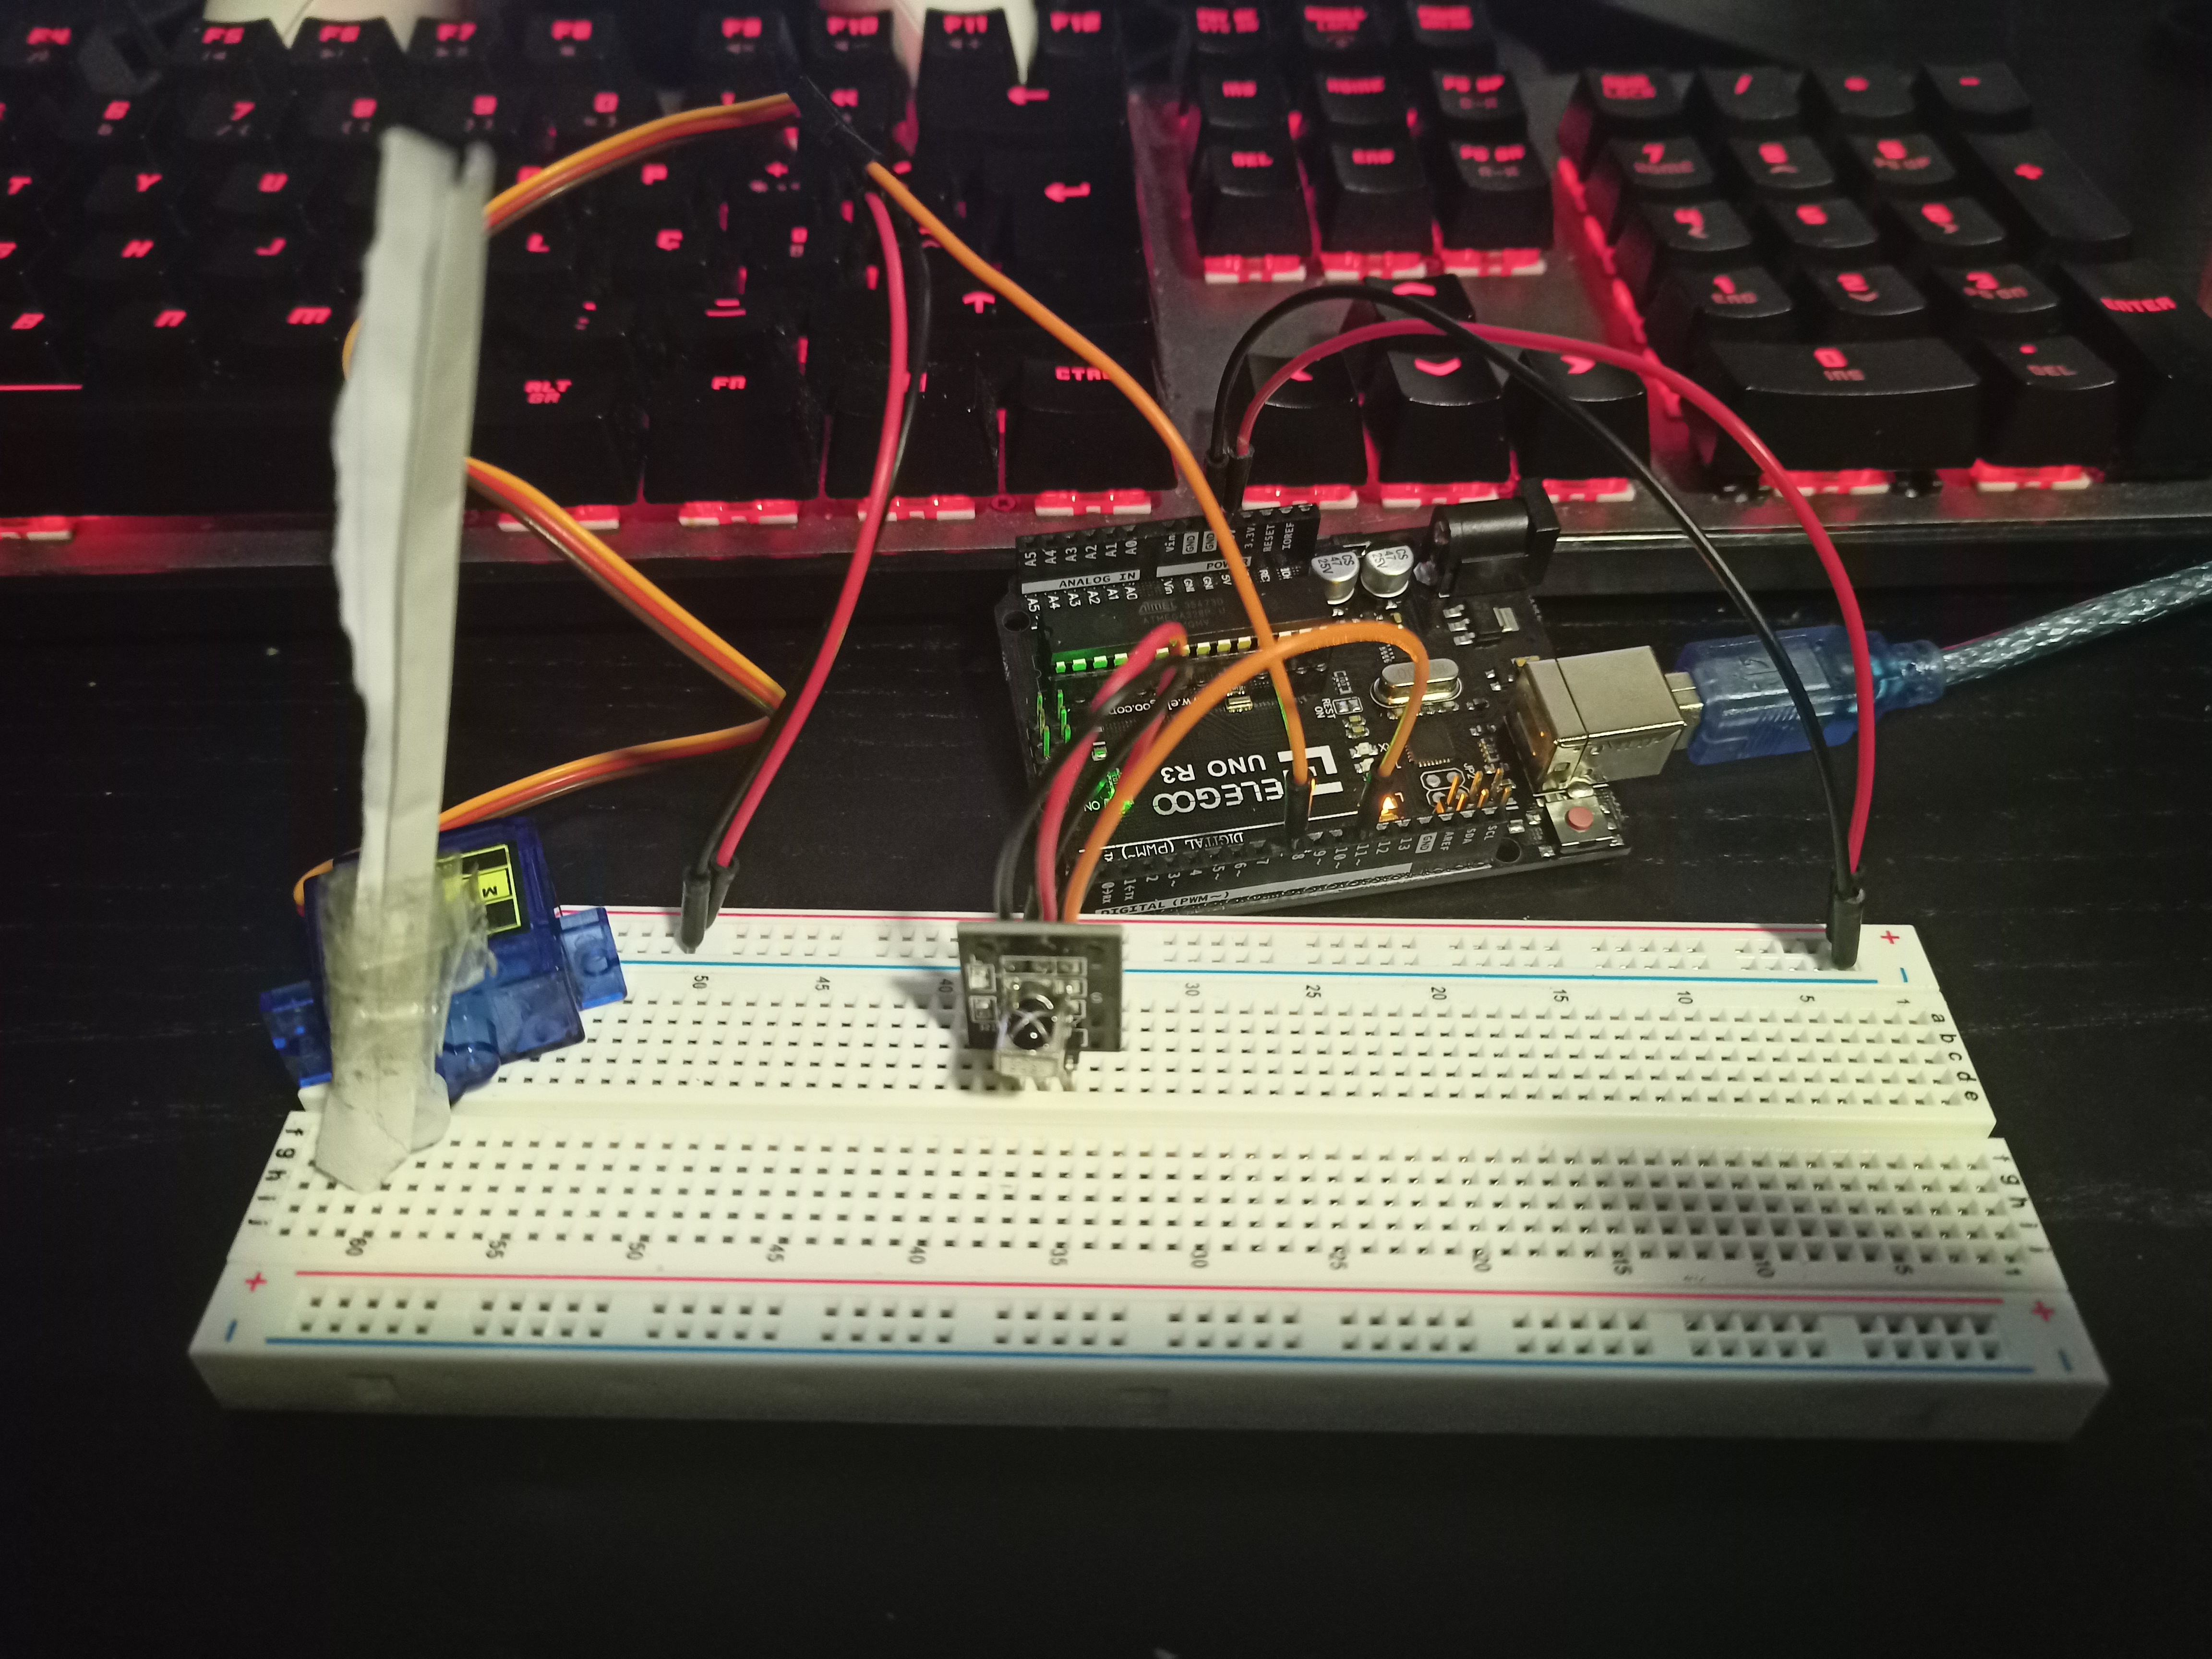
\includegraphics[scale=0.05]{images/hardware/sisC_IRL.jpg}
    \selectlanguage{portuguese}\caption{Esquema montado do Sistema A}
\end{figure}